% Options for packages loaded elsewhere
\PassOptionsToPackage{unicode}{hyperref}
\PassOptionsToPackage{hyphens}{url}
%
\documentclass[
  english,
  man]{apa6}
\usepackage{lmodern}
\usepackage{amsmath}
\usepackage{ifxetex,ifluatex}
\ifnum 0\ifxetex 1\fi\ifluatex 1\fi=0 % if pdftex
  \usepackage[T1]{fontenc}
  \usepackage[utf8]{inputenc}
  \usepackage{textcomp} % provide euro and other symbols
  \usepackage{amssymb}
\else % if luatex or xetex
  \usepackage{unicode-math}
  \defaultfontfeatures{Scale=MatchLowercase}
  \defaultfontfeatures[\rmfamily]{Ligatures=TeX,Scale=1}
\fi
% Use upquote if available, for straight quotes in verbatim environments
\IfFileExists{upquote.sty}{\usepackage{upquote}}{}
\IfFileExists{microtype.sty}{% use microtype if available
  \usepackage[]{microtype}
  \UseMicrotypeSet[protrusion]{basicmath} % disable protrusion for tt fonts
}{}
\makeatletter
\@ifundefined{KOMAClassName}{% if non-KOMA class
  \IfFileExists{parskip.sty}{%
    \usepackage{parskip}
  }{% else
    \setlength{\parindent}{0pt}
    \setlength{\parskip}{6pt plus 2pt minus 1pt}}
}{% if KOMA class
  \KOMAoptions{parskip=half}}
\makeatother
\usepackage{xcolor}
\IfFileExists{xurl.sty}{\usepackage{xurl}}{} % add URL line breaks if available
\IfFileExists{bookmark.sty}{\usepackage{bookmark}}{\usepackage{hyperref}}
\hypersetup{
  pdftitle={Frequency of code-switching in Romanian-Spanish bilinguals},
  pdfauthor={Gabriela Constantin-Dureci},
  pdflang={en-EN},
  hidelinks,
  pdfcreator={LaTeX via pandoc}}
\urlstyle{same} % disable monospaced font for URLs
\usepackage{longtable,booktabs}
\usepackage{calc} % for calculating minipage widths
% Correct order of tables after \paragraph or \subparagraph
\usepackage{etoolbox}
\makeatletter
\patchcmd\longtable{\par}{\if@noskipsec\mbox{}\fi\par}{}{}
\makeatother
% Allow footnotes in longtable head/foot
\IfFileExists{footnotehyper.sty}{\usepackage{footnotehyper}}{\usepackage{footnote}}
\makesavenoteenv{longtable}
\usepackage{graphicx}
\makeatletter
\def\maxwidth{\ifdim\Gin@nat@width>\linewidth\linewidth\else\Gin@nat@width\fi}
\def\maxheight{\ifdim\Gin@nat@height>\textheight\textheight\else\Gin@nat@height\fi}
\makeatother
% Scale images if necessary, so that they will not overflow the page
% margins by default, and it is still possible to overwrite the defaults
% using explicit options in \includegraphics[width, height, ...]{}
\setkeys{Gin}{width=\maxwidth,height=\maxheight,keepaspectratio}
% Set default figure placement to htbp
\makeatletter
\def\fps@figure{htbp}
\makeatother
\setlength{\emergencystretch}{3em} % prevent overfull lines
\providecommand{\tightlist}{%
  \setlength{\itemsep}{0pt}\setlength{\parskip}{0pt}}
\setcounter{secnumdepth}{-\maxdimen} % remove section numbering
% Make \paragraph and \subparagraph free-standing
\ifx\paragraph\undefined\else
  \let\oldparagraph\paragraph
  \renewcommand{\paragraph}[1]{\oldparagraph{#1}\mbox{}}
\fi
\ifx\subparagraph\undefined\else
  \let\oldsubparagraph\subparagraph
  \renewcommand{\subparagraph}[1]{\oldsubparagraph{#1}\mbox{}}
\fi
% Manuscript styling
\usepackage{upgreek}
\captionsetup{font=singlespacing,justification=justified}

% Table formatting
\usepackage{longtable}
\usepackage{lscape}
% \usepackage[counterclockwise]{rotating}   % Landscape page setup for large tables
\usepackage{multirow}		% Table styling
\usepackage{tabularx}		% Control Column width
\usepackage[flushleft]{threeparttable}	% Allows for three part tables with a specified notes section
\usepackage{threeparttablex}            % Lets threeparttable work with longtable

% Create new environments so endfloat can handle them
% \newenvironment{ltable}
%   {\begin{landscape}\begin{center}\begin{threeparttable}}
%   {\end{threeparttable}\end{center}\end{landscape}}
\newenvironment{lltable}{\begin{landscape}\begin{center}\begin{ThreePartTable}}{\end{ThreePartTable}\end{center}\end{landscape}}

% Enables adjusting longtable caption width to table width
% Solution found at http://golatex.de/longtable-mit-caption-so-breit-wie-die-tabelle-t15767.html
\makeatletter
\newcommand\LastLTentrywidth{1em}
\newlength\longtablewidth
\setlength{\longtablewidth}{1in}
\newcommand{\getlongtablewidth}{\begingroup \ifcsname LT@\roman{LT@tables}\endcsname \global\longtablewidth=0pt \renewcommand{\LT@entry}[2]{\global\advance\longtablewidth by ##2\relax\gdef\LastLTentrywidth{##2}}\@nameuse{LT@\roman{LT@tables}} \fi \endgroup}

% \setlength{\parindent}{0.5in}
% \setlength{\parskip}{0pt plus 0pt minus 0pt}

% \usepackage{etoolbox}
\makeatletter
\patchcmd{\HyOrg@maketitle}
  {\section{\normalfont\normalsize\abstractname}}
  {\section*{\normalfont\normalsize\abstractname}}
  {}{\typeout{Failed to patch abstract.}}
\patchcmd{\HyOrg@maketitle}
  {\section{\protect\normalfont{\@title}}}
  {\section*{\protect\normalfont{\@title}}}
  {}{\typeout{Failed to patch title.}}
\makeatother
\shorttitle{Final Paper, Data Science for Linguistics, Spring 2021}
\DeclareDelayedFloatFlavor{ThreePartTable}{table}
\DeclareDelayedFloatFlavor{lltable}{table}
\DeclareDelayedFloatFlavor*{longtable}{table}
\makeatletter
\renewcommand{\efloat@iwrite}[1]{\immediate\expandafter\protected@write\csname efloat@post#1\endcsname{}}
\makeatother
\usepackage{lineno}

\linenumbers
\usepackage{csquotes}
\ifxetex
  % Load polyglossia as late as possible: uses bidi with RTL langages (e.g. Hebrew, Arabic)
  \usepackage{polyglossia}
  \setmainlanguage[]{english}
\else
  \usepackage[shorthands=off,main=english]{babel}
\fi
\ifluatex
  \usepackage{selnolig}  % disable illegal ligatures
\fi
\newlength{\cslhangindent}
\setlength{\cslhangindent}{1.5em}
\newlength{\csllabelwidth}
\setlength{\csllabelwidth}{3em}
\newenvironment{CSLReferences}[2] % #1 hanging-ident, #2 entry spacing
 {% don't indent paragraphs
  \setlength{\parindent}{0pt}
  % turn on hanging indent if param 1 is 1
  \ifodd #1 \everypar{\setlength{\hangindent}{\cslhangindent}}\ignorespaces\fi
  % set entry spacing
  \ifnum #2 > 0
  \setlength{\parskip}{#2\baselineskip}
  \fi
 }%
 {}
\usepackage{calc}
\newcommand{\CSLBlock}[1]{#1\hfill\break}
\newcommand{\CSLLeftMargin}[1]{\parbox[t]{\csllabelwidth}{#1}}
\newcommand{\CSLRightInline}[1]{\parbox[t]{\linewidth - \csllabelwidth}{#1}\break}
\newcommand{\CSLIndent}[1]{\hspace{\cslhangindent}#1}

\title{Frequency of code-switching in Romanian-Spanish bilinguals}
\author{Gabriela Constantin-Dureci\textsuperscript{}}
\date{}


\affiliation{\phantom{0}}

\begin{document}
\maketitle

\hypertarget{introduction}{%
\section{Introduction}\label{introduction}}

\begin{itemize}
\item
  In this paper, I am focusing on a specific bilingual community, namely Romanian-Spanish bilinguals in Spain. Although there is a large community of Romanians in Spain, which leads to prevalent Romanian-Spanish bilingualism, studies on Romanian-Spanish bilinguals in Spain are scarce.
\item
  Code-switching (CS) is a common practice in bilingual communities across the world. In this paper, I am defining CS as the practice of using more than one language or language variety in discourse.
\item
  Labov' Gender Paradox is a sociolinguistic phenomenon which states that Women conform more closely than men to sociolinguistic norms that are overtly prescribed, but conform less than men when they are not.
  Women are more likely to use prestige forms and avoid stigmatized variants than men for a majority of linguistic variables, but that they are also more likely to lead language change by using innovative forms of variables.
  This sociolinguistic phenomenon is important for the present study, given that CS is considered a nonstandardized practice and is, therefore, stigmatized by prescriptive ideologies of language use.
\end{itemize}

\hypertarget{research-questions}{%
\section{Research Questions}\label{research-questions}}

\textbf{RQ 1.} Does gender influence frequency of CS?

\textbf{RQ 2.} Does generation status influence frequency of CS?

\textbf{RQ 3.} Does proficiency in Romanian influence frequency of CS?

\hypertarget{methods}{%
\section{Methods}\label{methods}}

In this section, I report my sample, materials, procedure, and data analysis.

\hypertarget{participants}{%
\subsection{Participants}\label{participants}}

One hundred eighty seven participants (72 female-identifying) completed this study. Since one of the research questions of this study targets bilinguals' generation status, the participants were further categorized in their respective groups. Specifically, one hundred and two participants belonged to the first generation (G1) group (41 female-identifying) and eighty five formed the second generation (G2) group (54 male-identifying).
Generation 1 (G1) bilinguals were born in Romania and immigrated to Spain as adults (i.e., after age 18) and Generation 2 (G2) bilinguals were born to at least one G1 parent. Therefore, G2 bilinguals could have either been born in Spain or born in Romania and immigrated to Spain before age 9 (see Torres and Potowski (2016)).

Descriptive statistics for the participant sample are offered in Table 1.

\begin{longtable}[]{@{}rrrr@{}}
\toprule
Generation & Proficiency\_Mean & Proficiency\_SD & Proficiency\_Range\tabularnewline
\midrule
\endhead
1 & 96.84811 & 1.549812 & 92.50384\tabularnewline
1 & 96.84811 & 1.549812 & 100.69086\tabularnewline
2 & 83.84732 & 4.432353 & 73.17738\tabularnewline
2 & 83.84732 & 4.432353 & 96.03021\tabularnewline
\bottomrule
\end{longtable}

\hypertarget{materials}{%
\subsection{Materials}\label{materials}}

\begin{itemize}
\item
  The short version of the Assessment of Code-Switching Experience Survey (ACSES; Blackburn (2013)) was used to assess participants' CS frequency. After reviewing their results on the ACSES, participants were further categorized as High frequency code-switchers (117 participants; 46 female-identifying; 52 G1) and Low frequency switchers (70 participants; 44 male-identifying; 20 G2).
\item
  Participants' proficiency was assessed via the Boston Naming Test (BNT; EF, Goodglass, and Weintraub (1983)) in Romanian.The BNT contains 60 outline drawings of objects and animals.
\item
  Participants also completed a Language History Questionnaire in order to gather socio-biographical data.
\end{itemize}

\hypertarget{procedure}{%
\subsection{Procedure}\label{procedure}}

Participants first completed the proficiency assessment, followed by the ACSES. The Language History Questionnaire was administered last.

\hypertarget{data-analysis}{%
\subsection{Data analysis}\label{data-analysis}}

The data were analyzed in R using a generalized linear mixed-effects model with a binomial linking function. The model included \emph{frequency of codeswitching} as the dependent variable and \emph{proficiency in Romanian}, \emph{generation status} and \emph{participants' gender} as fixed factors. High frequency of CS was coded as ``1'' and low frequency of CS was coded as ``0.'' Significance of main effects and all possible interactions were examined using hierarchical partitioning of the variance via nested model comparisons.

Lastly, I used R {[}Version 4.0.5; R Core Team (2020){]} and the R-package \emph{papaja} {[}Version 0.1.0.9997; Aust and Barth (2020){]} for all the analyses.

\hypertarget{results}{%
\section{Results}\label{results}}

The two panels in \emph{Figure 1} show the CS frequency of participants as a function of Romanian language proficiency, as well as generation (G1 or G2) and gender (female or male).
The model that examined frequency of CS as a factor of proficiency provided the best fit (with Pr(\textgreater Chi) = 0.0007759).
A visual analysis of the plots shows that for G1 participants, frequency of CS decreased as proficiency increased for both female and male participants. However, for G2 male participants, frequency of CS increased with proficiency, while for G2 female participants it decreased.

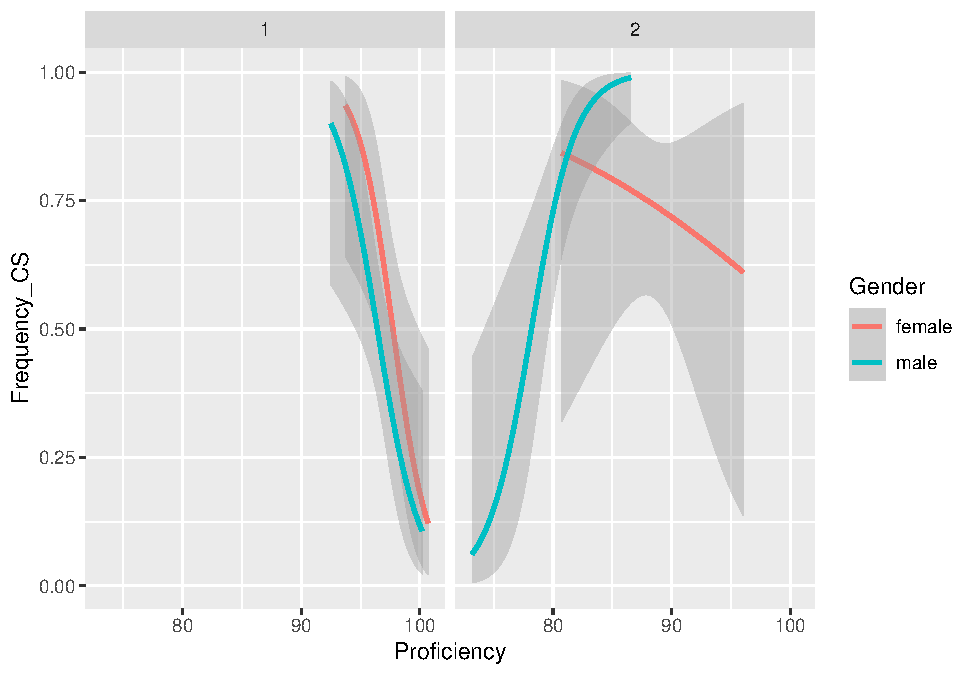
\includegraphics{Manuscript_files/figure-latex/unnamed-chunk-2-1.pdf}

\hypertarget{discussion}{%
\section{Discussion}\label{discussion}}

This study looked at Romanian-Spanish bilinguals' frequency of codeswitching and the potential influence of proficiency in Romanian, gender identity, and generation status.

\newpage

\hypertarget{references}{%
\section{References}\label{references}}

\begingroup
\setlength{\parindent}{-0.5in}
\setlength{\leftskip}{0.5in}

\hypertarget{refs}{}
\begin{CSLReferences}{1}{0}
\leavevmode\hypertarget{ref-R-papaja}{}%
Aust, F., \& Barth, M. (2020). \emph{{papaja}: {Create} {APA} manuscripts with {R Markdown}}. Retrieved from \url{https://github.com/crsh/papaja}

\leavevmode\hypertarget{ref-phdthesis}{}%
Blackburn, A. (2013). \emph{A study of the relationship between code switching and the bilingual advantage: Evidence that language use modulates neural indices of language processing and cognitive control} (PhD thesis).

\leavevmode\hypertarget{ref-article}{}%
EF, K., Goodglass, H., \& Weintraub, S. (1983). Boston naming test. \emph{Brain and LanguageJournal of Speech \& Hearing ResearchThe Clinical Neuropsychologist}. \url{https://doi.org/10.1037/t27208-000}

\leavevmode\hypertarget{ref-R-base}{}%
R Core Team. (2020). \emph{R: A language and environment for statistical computing}. Vienna, Austria: R Foundation for Statistical Computing. Retrieved from \url{https://www.R-project.org/}

\leavevmode\hypertarget{ref-inbook}{}%
Torres, L., \& Potowski, K. (2016). Hablamos los dos in the windy city: Codeswitching among puerto ricans, mexicans and MexiRicans in chicago (pp. 83--105). \url{https://doi.org/10.1075/ihll.11.04tor}

\end{CSLReferences}

\endgroup


\end{document}
